%! suppress = Unicode
\chapter{ПРАКТИЧЕСКАЯ РЕАЛИЗАЦИЯ СЕРВИСА}\label{ch:ch3-implementation}

В данной главе будет рассмотрен процесс выбора технологий и планирования архитектуры системы, в которой будет использоваться предлагаемая технология, а также внутренняя архитектура самой реализации.

% TODO описать планирование архитектуры системы

\section{Требования к реализации}\label{sec:implementation-requirements}

Спецификация, описанная в главе 2, не указывает единственный разрешённый источник для получения маппингов.
Источником может быть реляционная или нереляционная база данных, система контроля версий, расположенный локально в файловой системе файл, специализированный веб-сервер для получения настроек, или любое другое хранилище данных.
Кроме того, сам формат маппингов не является строго определённым, так как они могут храниться в различных источниках.
Таким образом, формат хранения настроек
В спецификации не определяется ожидаемое поведение системы при получении каких-либо ошибок со стороны GraphQL-сервера.
Также не ограничивается список технологий, которые могут быть использованы для трансформации ответа в формате JSON\@.
Таким образом, для данной реализации необходимо определить детали требований, которые будут использоваться при проверке его работоспособности и апробации.

Определим список свойств и особенностей данной, выбранных для данной реализации, следующим образом:
\begin{itemize}
	\item Маппинги указываются в системе контроля версий GIT
	\item По умолчанию берутся из локально расположенного текстового файла
	\item В качестве формата для маппингов используется формат YAML;
	% \item при перенаправлении запроса к другому эндпоинту обрабатывает только успешные ответы от этого эндпоинта;
	% \item Сервис не осуществляет трансформирование ответа в формате JSON, полученного от GraphQL-сервиса;
	\item В случае получения ответа с кодом ответа HTTP отличным от кода 200 (успешный ответ), ответ передаётся клиенту в неизменном виде.
	\item
\end{itemize}



\section{Выбор технологий}\label{sec:choose-technology}

Для системы, реализуемой в рамках выпускной квалификационной работы, в дальнейшем будет использоваться название R2G (Rest to GraphQL).

Для создания системы будет использован Spring Framework, являющийся одним из самых распространённых и мощных фреймворков для создания веб-сервисов.
Spring Framework включает в себя множество различных модулей, которые позволяют значительно ускорить разработку и уменьшить количество необходимого кода за счёт использования многочисленных дополнительных модулей.
В частности, будут использованы следующие модули:

\begin{itemize}
	\item Spring Boot позволяет подключать так называемые стартеры (starters), которые включают в себя другие модули и упрощают их конфигурирование.
	За счёт использования стартеров значительно сокращается объём необходимой работы.

	\item Spring Web используется для создания эндпоинтов для обработки входящих REST-запросов. % Можно заменить на WebFlux
	Данная технология позволяет задать точки входа в веб-сервис, а также предоставляет функциональность для обработки входящих запросов.

	\item Spring Cloud Config для управления настройками сервиса, в частности для возможности получения настроек и маппингов из GIT-репозитория.
\end{itemize}

Spring Framework изначально разрабатывался для использования с языком Java, однако на данный момент поддерживает значительное число языков JVM, и в рамках данной работы будет использован язык Kotlin, имеющий среди преимуществ перед Java лаконичность и возможность использования корутин (coroutine, легковесных потоков) для повышения производительности при использовании многопоточной обработки запросов.
Также при использовании языка Kotlin упрощается использование реактивной парадигмы программирования.
Достоинством этого подхода при создании информационной системы является поддержка неблокирующего ввода/вывода, за счёт которого увеличивается количество запросов, которые сервис может обрабатывать параллельно.
Таким образом увеличивается скорость обработки запросов при высокой нагрузке на веб-сервис, а также имеющиеся ресурсы утилизируется более эффективно.

Для взаимодействия с GraphQL-сервисами существуют специальные библиотеки, как например Apollo Client, позволяющие упростить создание клиентских приложений за счёт генерации кода на основании схемы и GraphQL-запросов.
Однако подобный подход неприменим в данном случае, так как разрабатываемый сервис должен уметь работать с GraphQL-сервисами в общем случае.
Поэтому для обращения к GraphQL-сервисам будет использован обычный HTTP-клиент.
В качестве одного из HTTP-клиентов Spring Framework предоставляет технологию WebClient, который позволяет применить ранее упомянутый неблокирующий ввод/вывод, как следствие мы получаем все его достоинства.

Для преобразования результатов используем технологию JOLT, так как она является достаточно мощной технологией, позволяющей осуществлять разнообразные манипуляции с JSON, позволяет писать юнит-тесты для проверки написанных преобразований.
Кроме того, JOLT является одной из немногих подобных технологий имеет реализацию в виде библиотеки для Java.


\section{Обзор исходных кодов реализации}\label{sec:sources-review}

Исходный код прототипа содержит ряд пакетов, логически разделяющих классы.
Каждый пакет представляет из себя уровень абстракции над действиями, выполняемыми сервисом при обработке запросов.
Исходные коды классов приведены в приложении 8.

При описании реализации будет использоваться термин bean (бин), который обозначает некий объект, которым управляет Spring Framework.
Во многих случаях термины бин и объект являются взаимозаменяемыми.

На \firef{fig:ch3-classes} изображено дерево пакетов модуля main, содержащего исходные коды приложения.

\begin{figure}[ht!]
	\center
	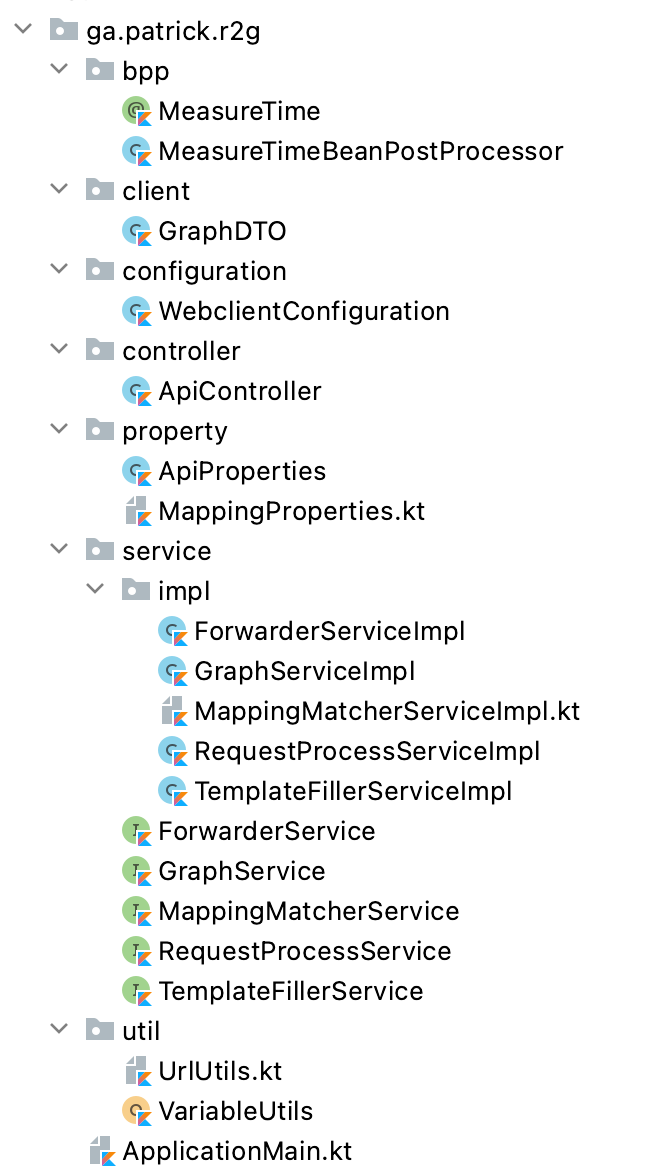
\includegraphics [scale=0.6] {my_folder/images/ch3-classes}
	\caption{Дерево пакетов модуля main}
	\label{fig:ch3-classes}
\end{figure}

\subsection{Пакет controller}\label{subsec:package-controller}

Данный пакет традиционно включает в себя классы, ответственные за принятие запроса к сервису и отправку ответа.
Каждый класс содержит набор методов с указаниями о том, какие запросы данный метод обрабатывает, и какие данные требуются для его работы.
Данные указания обычно даются в виде аннотаций.

Этот пакет имеет единственный класс ApiController, имеющий единственный метод endpoint.
Аннотация \texttt{@RequestMapping("/**")} указывает на то, что данный метод принимает запросы с любыми \texttt{path} и \texttt{method} (\texttt{GET}, \texttt{POST} и прочие).
Также, данный метод принимает в качестве аргумента объект \texttt{HttpServletRequest}, который содержит информацию о пришедшем запросе, такую как \texttt{path}, \texttt{method}, параметры \texttt{query}, тело запроса, словарь заголовков.
Таким образом, при получении любого запроса к данному веб-сервису информация об этом запросе будет передана в качестве аргументов при вызове этого метода.
Метод не имеет никакой логики, кроме вызова метода \texttt{processRequest} объекта \texttt{RequestProcessService}, который будет рассмотрен далее.

\subsection{Пакет service}\label{subsec:package-service}

Данный пакет включает в себя классы, ответственные за так называемую бизнес-логику.
В корне данного пакета находится ряд интерфейсов.
Интерфейсы используются в качестве контрактов для сервисов, которые планируется реализовать.
Подход, при котором сначала создаются интерфейсы, и только затем имплементации, широко используется при использовании Test Driven Development.
При использовании этого подхода котором прежде чем приступить к реализации продумывается внутренняя архитектура системы, создаются классы-интерфейсы, и для них пишутся тестовые сценарии, описывающие ожидаемое поведение системы.
Затем, классы, реализующие эти интерфейсы, помещяются в отдельных файлах, обычно в подпакетах с названием impl и именем, состоящим из названия интерфейса и постфикса Impl.
Также, данный подход позволяет создавать несколько реализаций для каждого интерфейса, позволяя подменять эти реализации перед запуском с помощью файла настроек, или даже в процессе работы программы.
Также, использование интерфейсов позволяет немного увеличить производительность и ускорить автоматизированное тестирование за счёт использования механизмов динамического проксирования JDK (Java Developer Kit), вместо технологии CGLIB\@.
Обе технологии используются для создания так называемых Proxy-объектов и Mock-объектов.

Proxy-объекты используются для неявного применения дополнительного поведения к какому-либо классу или методу, а также при использовании парадигмы АОП (Аспектно-ориентированное программирование).
Например, Proxy-объекты могут использоваться для кеширования ответа какого-либо метода, логирования аргументов и ответов методов, или для подсчёта времени выполнения метода.
В частности, последнее применение будет описано далее при обзоре аннотации \texttt{@MeasureTime} и класса \texttt{MeasureTimeBeanPostProcessor}.

Mock-объекты используются для эмуляции поведения какого-либо объекта в процессе проведения автоматизированного тестирования.
Например, какой-либо сервис в процессе своей работы осуществляет обращение к базе данных через некий бин.
Создание, наполнение и очистка базы данных для каждого теста являются значительными накладными расходами.
А в случае с сетевыми вызовами в большинстве случаев использование реального обращения к внешним сервисам (например, на тестовом или разработческом стенде) является либо невозможным, либо слишком медленным.
Кроме того, согласно методологии тестирования модули программы должны быть протестированы отдельно.
Поэтому для модульных (компонентных) тестов реализация зависимого бина подменяется Mock-объектом, для которого вручную задаётся определённое поведение.
Например, если бин получил в качестве аргумента строку \texttt{"a"}, то он должен будет ответить строкой \texttt{"b"}.
Применение Mock-объектов будет продемонстрировано в обзоре модуля \texttt{test}.

Технология CGLIB является более медленной, чем механизм динамического проксирования JDK, но механизм JDK работает за счёт реализации тех же интерфейсов, что и исходный класс.
Соответственно, для использования этого механизма JDK наш проксируемый/мокируемый класс должен реализовывать некий интерфейс.


Рассмотрим интерфейсы пакета service.
Согласно принципу Single Responsibility, каждый компонент имеет строгую зону ответственности.
Ответственность каждого из них описана ниже:

\begin{itemize}
	\item RequestProcessService -- является ключевым компонентом системы.
	Имеет единственный метод \texttt{processRequest}, который принимает объект входящего запроса \texttt{HttpServletRequest} и осуществляет отправку исходящего запроса к нужному сервису.
	В частности, этот метод получает соответствующий запросу маппинг, и в случае успеха формирует и отправляет запрос к соответствующему GraphQL-сервису.
	А в случае, если маппинг не был найден, перенаправляет запрос к некому серверу по умолчанию, указанному в настройках.

	\item MappingMatcherService -- используется для поиска маппинга, соответствующего входящему запросу.
	Он имеет единственный метод \texttt{findMapping}, который принимает объект запроса \texttt{HttpServletRequest}, находит и отдаёт соответствующий ему маппинг из настроек.

	\item TemplateFillerService – заполняет шаблон GraphQL-запроса параметрами, полученными из входящего запроса, в соответствии с маппингом.
	Компонент получает значения переменных для заполнения из URI, query parameters и тела запроса.

	\item GraphService – осуществляет отправку GraphQL-запроса.
	Имеет единственный метод send, принимающий URL запрашиваемого сервиса и объект GraphDTO, который будет отправлен в GraphQL-сервис.

	\item ForwarderService – перенаправляет запросы, для которых не нашлось маппинга, в Gateway API, указанный в настройках.
	Имеет единственный метод send, принимающий объект \texttt{HttpServletRequest}.
	Запрос передаётся с сохранением URI, headers, query parameters, тела и прочих параметров входящего запроса в исходном виде.

\end{itemize}

% Если маппинг не был найден, то он передаёт объект запроса в ForwarderService и возвращает ответ, полученный от Gateway API. Если маппинг был найден, то он использует TemplateFillerService для создания GraphQL-запроса, выполняет его с помощью GraphClient, который будет рассмотрен далее, и возвращает полученный ответ пользователю.


\subsection{Пакет util}\label{subsec:package-util}

Данный пакет включает в себя единственный класс VariableUtils, который содержит утилитарные методы для:

\begin{itemize}
	\item получения маски маппинга, которая будет использована для сравнения с пришедшим запросом;
	\item получения списка переменных, которые ожидается найти в пришедшем запросе;
	\item получения значения переменных из пришедшего запроса.
\end{itemize}

Для получения значений из тела запроса, представляющего из себя JSON, использована библиотека JsonPath.

\subsection{Пакет property}

Данный пакет содержит файл MappingProperties, содержащий следующие классы, по своей структуре повторяющие структуру маппингов, записанных в виде YAML-файла (например, application.yml):

\begin{itemize}
	\item MappingProperties -- корневой класс настроек.
	Он имеет в себе следующие поля:
		\subitem defaultEndpoint -- URL эндпоинта по умолчанию
		\subitem mappings -- список объектов типа Mapping, каждый из которых представляет собой описание правила для маппинга входящего запроса к исходящему, а также правило преобразования ответа.
		\subitem endpoints -- список доступных GraphQL-серверов.
		В этом списке указываются псевдонимы для URL этих серверов, чтобы избежать их многократного дублирования в маппингах.

	\item Mapping -- описание правила для маппинга входящего запроса к исходящему:
		\subitem path -- шаблон пути, который может содержать переменные;
		\subitem methods -- HTTP методы запроса;
		\subitem endpointName -- псевдоним GraphQL-сервера, на который нужно отправить запрос;
		\subitem template -- шаблон для запроса, представляющий собой GraphQL-запрос, возможно, содержащий в себе переменные, которые будут заполнены с помощью данных из входящего запроса.
		\subitem variables -- список объектов Variable -- описаний переменных, поддерживаемых GraphQL, которые используются в шаблоне, и значения для которых мы также получаем из входящего запроса.

	\item Endpoint -- объект, содержащий два поля:
		\subitem name -- псевдоним GraphQL-сервера;
		\subitem uri -- адрес этого сервера.

	\item VariableDefinition -- список переменных, которые следует отправить в составе GraphQL-запроса.
		\subitem name -- название переменной, используемой в GraphQL-запросе;
		\subitem source -- данные для получения значения этой переменной из входящего запроса;
		\subitem type -- тип данных переменной.
			Возможные значения содержатся в перечислении GraphVariableType.

	\item GraphVariableType -- набор возможных типов переменных.
		На данный момент поддерживаются строковые, целочисленные и дробные переменные.

\end{itemize}

\subsection{Пакет bpp}\label{subsec:package-bpp}

Данный пакет включает в себя класс \texttt{MeasureTimeBeanPostProcessor} и аннотацию \texttt{MeasureTime}.
Аннотация создана для замера скорости выполнения запроса, и должна быть поставлена на классе, скорость выполнения функций которого нас интересует.
Результаты использования этой аннотации будут более подробно рассмотрены в главе 4. % TODO ссылка

В данный момент эта аннотация стоит на классах \texttt{RequestProcessServiceImpl} и \texttt{GraphServiceImpl}. % TODO актуализировать
Соответственно, мы сможем засечь время выполнения функции \texttt{processRequest} и вычесть из него время выполнения фунции \texttt{send}, таким образом получив чистое время обработки запроса кодом приложения.

Класс \texttt{MeasureTimeBeanPostProcessor} отвечает за имплементацию логики засекания времени выполнения функций для классов, над которыми установлена аннотация \texttt{MeasureTime}.
Он является имплементацией \texttt{BeanPostProcessor}, которые в Spring Framework нужны для донастройки созданных бинов на разных этапах инициализации приложения.

Функция \texttt{postProcessBeforeInitialization} выполняется первой, и объект, который передаётся в качестве аргумента к этой фунции, является оригинальным бином (а не Proxy-объектом).
Вторым аргументом фунции является название (уникальный идентификатор) бина.
С помощью него мы сможем найти оригинальное описание класса, из которого был создан оригинальный бин.
Записываем название бина и информацию о его типе в словарь.

Функция \texttt{postProcessBeforeInitialization} выполняется второй.
Объект, получаемый в качестве аргумента, уже необязательно является оригинальным бином, а может являться Proxy-объектом, созданным другим \texttt{BeanPostProcessor}.
В свою очередь, Proxy-объекты могут не содержать всю нужную информацию, в частности, информацию об аннотациях, установленных над классом, его методами и полями.
Получаем информацию об оригинальном классе из словаря по имени бина.
Чтобы замерить время выполнения метода, создадим Proxy-объект, и зададим поведение для каждого метода.
При вызове каждого метода будем получать текущее системное время в миллисекундах, затем выполнять оригинальный метод проксируемого объекта, и после этого снова получать текущее системное время.
Вычтя из второго первое, получим время выполнения метода.
Запишем результат выполнения в словарь для последующей обработки, и также выведем в стандартный вывод (консоль).

\subsection{Модуль test}\label{subsec:module-test}

На \firef{fig:ch3-tests} изображено дерево пакетов модуля tests, содержащего исходные коды тестов, использующихся для автоматизированной проверки работоспособности приложения в целом, а также его компонентов по отдельности.

\begin{figure}[ht!]
	\center
	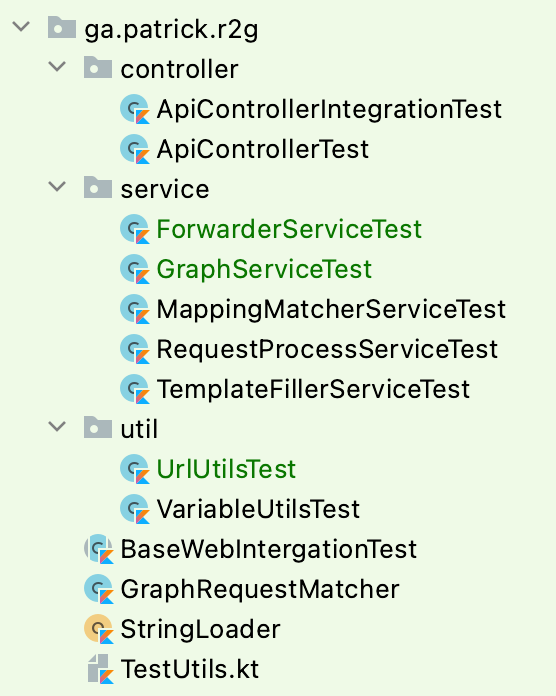
\includegraphics [scale=0.6] {my_folder/images/ch3-tests}
	\caption{Дерево пакетов модуля test}
	\label{fig:ch3-tests}
\end{figure}

% Рассмотрим тестовые классы более подробно: % ещё выше обещал рассказать про Mock'и

%\begin{itemize}

Данный модуль содержит в себе юнит-тесты для проверки работы ряда компоне, а также несколько интеграционных сервисов, проверяющих работоспособность системы вцелом.

Интеграционные тесты утилизируют тестовые данные, подготовленные ранее %в разделе 2.3
, причём вместо вызова внешних систем реализуются заглушки с помощью технологии WireMock, позволяющей указать ожидаемый запрос и соответствующий ему ответ.


\section{Выводы} \label{sec:ch3-conclusion}

В данной главе были поставлены требования к реализации системы, сформулированные на основании спецификации, описанной в теоретической части работы.
Были перечислены использованные технологии и представлены причины их выбора, и затем был приведён обзор исходного кода и разобраны некоторые примечательные детали реализации.
